\documentclass[12pt, a4paper]{article}
\usepackage{ctex} % 中文的宏包
\usepackage{indentfirst}
%\usepackage{graphicx} % 插入圖片的宏包
%\usepackage{float} % 設置圖片浮動位置的宏包
%\usepackage{subfigure} % 插入多圖時用子圖顯示宏包
\usepackage{listings} % 代碼塊宏包
\usepackage{color} % 代碼高亮
\usepackage[colorlinks,linkcolor=blue]{hyperref} % URL 包
%\usepackage[pdf]{graphviz}
\usepackage{tikz}

\usetikzlibrary{automata, positioning, arrows}

\definecolor{dkgreen}{rgb}{0,0.6,0}
\definecolor{gray}{rgb}{0.5,0.5,0.5}
\definecolor{mauve}{rgb}{0.58,0,0.82}

\lstset{ %
    %language=Octave,                % the language of the code
    basicstyle=\scriptsize\Hack,           % the size of the fonts that are used for the code
    numbers=none,                   % where to put the line-numbers
    numberstyle=\tiny\color{gray},  % the style that is used for the line-numbers
    stepnumber=2,                   % the step between two line-numbers. If it's 1, each line 
                                    % will be numbered
    numbersep=3pt,                  % how far the line-numbers are from the code
    backgroundcolor=\color{white},      % choose the background color. You must add \usepackage{color}
    showspaces=false,               % show spaces adding particular underscores
    showstringspaces=false,         % underline spaces within strings
    showtabs=false,                 % show tabs within strings adding particular underscores
    frame=single,                   % adds a frame around the code
    rulecolor=\color{black},        % if not set, the frame-color may be changed on line-breaks within not-black text (e.g. commens (green here))
    tabsize=2,                      % sets default tabsize to 2 spaces
    captionpos=b,                   % sets the caption-position to bottom
    breaklines=true,                % sets automatic line breaking
    breakatwhitespace=false,        % sets if automatic breaks should only happen at whitespace
    title=\lstname,                   % show the filename of files included with \lstinputlisting;
                                    % also try caption instead of title
    keywordstyle=\color{blue},          % keyword style
    commentstyle=\color{dkgreen},       % comment style
    stringstyle=\color{mauve},         % string literal style
    escapeinside={\%*}{*},            % if you want to add LaTeX within your code
    morekeywords={*,...}               % if you want to add more keywords to the set
}
\setCJKmainfont{Noto Serif CJK TC} % 主要字體 Noto Serif
\newfontfamily\Hack{Hack} % 代碼字體
\author{軟件 1804 8209180438 黃柏曛}
\date{\today}
\title{編譯原理 教材第 63 頁 3 6 7 9 12 題}
\begin{document}
\maketitle
\section{P63 第 3 题}
    \subsection{使用 C 或是 Pascal 的语言编写过程 GetChar、GetBC 和 Concat}

    \subsubsection{GetChar}
    \begin{lstlisting}[language=Octave]
    void Getchar() 
    {
      if(flag == 0)
      {
        if((fp = fopen("1.txt","r")) == NULL)
        {
          printf("cannot open this file\n");
          exit(0);
        }
      }
      flag++;

      character = fgetc(fp);

      if(character == EOF) {
        fclose(fp);
      }
    }
    \end{lstlisting}
    \subsubsection{GetBC}
    \begin{lstlisting}[language=Octave]
    void Getbc()
    {
      if(character == EOF)
        return;
      while(character == ' ' || character == '\n' || character == '\t')
       Getchar();
    }
    \end{lstlisting}

    \subsubsection{Concat}
    \begin{lstlisting}[language=Octave]
    void Concat()
    {
      if(i == 0)
      {
        token[0] = character;
        token[1] = '/0';
        i = 1;
      }
      else
      {
        token[i] = character;
        i++;
        token[i] = '/0';
      }
    }
    \end{lstlisting}
    
\section{P63 第 6 题}
    \subsection{令 A、B 和 C 是任意正规式,证明以下关系成立}

    {$A \mid A = A$}

    {$(A^{\star})^{\star} = A^{\star}$}

    {$A^{\star} = \varepsilon \mid AA^{\star}$}

    {$(AB)^{\star}A = A(BA)^{\star}$}

    {$(A \mid B)^{\star} = (A^{\star}B^{\star})^{\star} = (A^{\star} \mid B^{\star})^{\star}$}

    {$A = b \mid aA$ 当且仅当 $A = a^{\star}b$}

    %{解:}
    % 1
    \subsubsection{$A \mid A = A$}

    {抽取律}
    
    {$L(A \mid A) = L(A) \cup L(A) = L(A)$}
    % 2
    \subsubsection{$(A^{\star})^{\star} = A^{\star}$}

    {证:}\\

    {$L(A^{\star}\cdot A^{\star}\cdots A^{\star}) = L(A^{\star})$}

    {$\Longleftrightarrow L(A \cdot A \cdot A \cdots A) = L(A \cdots A)$}

    {$\Longleftrightarrow L(A^{\star}) = L((A^{\star})^{\star})$}

    %3
    \subsubsection{$A^{\star} = \varepsilon \mid AA^{\star}$}

    {证:}\\

    {$L(\varepsilon \mid AA^{\star}) = L(\varepsilon) \cup L(A)L(A^{\star})$}

    {$= L(\varepsilon) \cup L(A)(L(A))^{\star}$}

    {$= L(\varepsilon) \cup L(A) \cup (L(A))\cup\cdots\cup\cdots$}

    {$= (L(A))^{\star} = L(A^{\star})$}\\

    {综合上述,所以原式成立。}

    %4
    \subsubsection{$(AB)^{\star}A = A(BA)^{\star}$}
  
    {证:}\\

    {$((AB^{0})\mid(AB^{1})\cdots((AB)^{N}))\cdot A = \varepsilon A \mid A \cdot (AB)^{1}\cdots$}

    {$= A \cdot \varepsilon \mid A(BA)^{1} \mid \cdots$}

    {$= A(BA)^{\star}$}
    %5
    \subsubsection{$(A \mid B)^{\star} = (A^{\star}B^{\star})^{\star} = (A^{\star} \mid B^{\star})^{\star}$}

    {证:}\\

    {证明 $(A \mid B)^{\star} = (A^{\star}B^{\star})^{\star}$}

    {$L(A) \subseteq L(A^{\star})L(B^{\star})$}

    {$L(B) \subseteq L(A^{\star})L(B^{\star})$}

    {$L(A) \cup L(B) \subseteq L(A^{\star})L(B^{\star})$}

    {$(L(A) \cup L(B))^{\star} \subseteq (L(A^{\star})L(B^{\star}))^{\star}$}

    {又 ${}^\cdot{}_\cdot{}^\cdot L(A) \subseteq L(A) \cup L(B)$}

    {\qquad$L(B) \subseteq L(A) \cup L(B)$}

    {${}_\cdot{}^\cdot{}_\cdot L(A)^{\star}\cdot L(B^{\star}) \subseteq ((L(A) \cup L(B))^{\star})^{2}$}

    {\quad$L(A)^{\star}\cdot L(B^{\star}) \subseteq (L(A) \cup L(B))^{\star}$}

    {\quad$(L(A)^{\star}\cdot L(B^{\star}))^{\star} \subseteq (L(A) \cup L(B))^{\star}$}

    {${}_\cdot{}^\cdot{}_\cdot (L(A) \cdot L(B))^{\star} = (L(A^{\star}) \cup L(B^{\star}))^{\star}$}

    \textbf{${}_\cdot{}^\cdot{}_\cdot (A \mid B)^{\star} = (A^{\star}B^{\star})^{\star}$ 成立}\\

    {证明 $(A \mid B)^{\star} = (A^{\star} \mid B^{\star})^{\star}$}

    {$L(A) \subseteq L(A^{\star}) \cup L(B^{\star})$}

    {$L(B) \subseteq L(A^{\star}) \cup L(B^{\star})$}

    {$L(A) \cup L(B) \subseteq L(A^{\star}) \cup L(B^{\star})$}

    {$(L(A) \cup L(B) \subseteq (L(A^{\star}))^{\star} \cup L(B^{\star}))^{\star}$}

    {又 ${}^\cdot{}_\cdot{}^\cdot L(A^{\star}) \subseteq (L(A) \cup L(B))^{\star}$}

    {\qquad$L(B^{\star}) \subseteq (L(A) \cup L(B))^{\star}$}

    {$(L(A^{\star}) \cup L(B^{\star}))^{\star} \subseteq (L(A) \cup L(B))^{\star}$}\\

    \textbf{综合上述 ${}_\cdot{}^\cdot{}_\cdot (A \mid B)^{\star} = (A^{\star} \mid B^{\star})^{\star}$ 成立}

    \textbf{所以原式成立}

    %6
    \subsubsection{$A = b \mid aA$ 当且仅当 $A = a^{\star}b$}

    {若 $A = a^{\star}b$ 则 $A = b \mid aA$}\\

    {$L(A) = L(a)^{\star}L(b)$}

    {\qquad\, $ = L(\varepsilon)L(b) \cup L(a)^{\star}L(b)$}

    {\qquad\, $ = L(b) \cup L(a)^{\star}L(b)$}

    {\qquad\, $ = L(b) \cup L(a)L(a)^{\star}L(b)$}

    {\qquad\, $ = L(b \mid aA)$}

    {再证当 $A = b \mid aA$ 则 $A = a^{\star}b$}

    {$L(A) = L(b) \cup L(aA)$}

    {\qquad\, $ = L(b)L(\varepsilon) \cup L(a)L(A)$}

    {\qquad\, $ = L(a)^{\star}L(b)$}\\

    \textbf{综上原式成立}

\section{P63 第 7 题}
    \subsection{构造下列正则相应的 DFA}

    {$1(0 \mid 1)^{\star}101$}

    {$1(1010^{\star}11(010)^{\star}1)^{\star}0$}

    {$0^{\star}10^{\star}10^{\star}10^{\star}$}

    {$(00 \mid 11)^{\star}((01 \mid 10)(00 \mid 11)^{\star}(01 \mid 10)(00 \mid 11)^{\star})^{\star}$}

      %1
      \subsubsection{$1(0 \mid 1)^{\star}101$}

      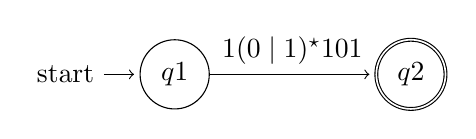
\begin{tikzpicture}[shorten >=2pt,node distance=3cm,on grid,auto] 
        \node[state,initial] (q_1) {$q1$};  
        \node[state,accepting](q_2) [right=of q_1] {$q2$};
        \path[->]
        (q_1) edge node {$1(0 \mid 1)^{\star}101$} (q_2);
        
      \end{tikzpicture}

      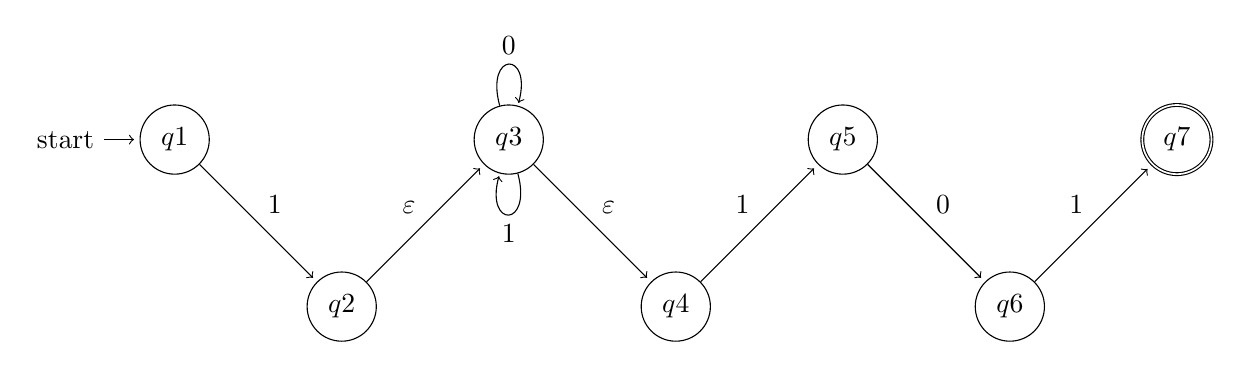
\begin{tikzpicture}[shorten >=2pt,node distance=3cm,on grid,auto] 
        \node[state,initial] (q_1) {$q1$};  
        \node[state](q_2) [below right=of q_1] {$q2$};
        \node[state](q_3) [above right=of q_2] {$q3$};
        \node[state](q_4) [below right=of q_3] {$q4$};
        \node[state](q_5) [above right=of q_4] {$q5$};
        \node[state](q_6) [below right=of q_5] {$q6$};
        \node[state,accepting](q_7) [above right=of q_6] {$q7$};
        \path[->]
        (q_1) edge node {$1$} (q_2)
        (q_2) edge node {$\varepsilon$} (q_3)
        (q_3) edge node {$\varepsilon$} (q_4)
              edge [loop above] node {$0$} ()
              edge [loop below] node {$1$} ()
        (q_4) edge node {$1$} (q_5)
        (q_5) edge node {$0$} (q_6)
        (q_6) edge node {$1$} (q_7);
      \end{tikzpicture}

      %2
      \subsubsection{$1(1010^{\star}11(010)^{\star}1)^{\star}0$}

      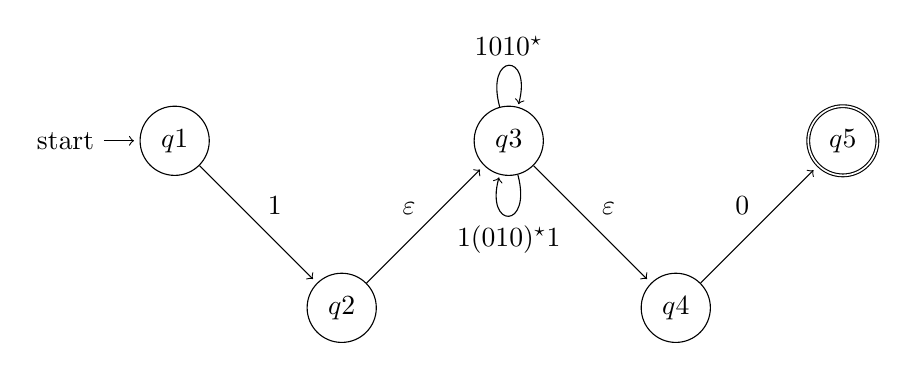
\begin{tikzpicture}[shorten >=2pt,node distance=3cm,on grid,auto] 
        \node[state,initial] (q_1) {$q1$};  
        \node[state](q_2) [below right=of q_1] {$q2$};
        \node[state](q_3) [above right=of q_2] {$q3$};
        \node[state](q_4) [below right=of q_3] {$q4$};
        \node[state,accepting](q_5) [above right=of q_4] {$q5$};
        \path[->]
        (q_1) edge node {$1$} (q_2)
        (q_2) edge node {$\varepsilon$} (q_3)
        (q_3) edge node {$\varepsilon$} (q_4)
              edge [loop above] node {$1010^{\star}$} ()
              edge [loop below] node {$1(010)^{\star}1$} ()
        (q_4) edge node {$0$} (q_5);
      \end{tikzpicture}

      %3
      \subsubsection{$0^{\star}10^{\star}10^{\star}10^{\star}$}

      \begin{tikzpicture}[shorten >=2pt,node distance=3cm,on grid,auto] 
        \node[state,initial] (q_1) {$q1$};  
        \node[state](q_2) [right=of q_1] {$q2$};
        \node[state](q_3) [right=of q_2] {$q3$};
        \node[state](q_4) [right=of q_3] {$q4$};
        \node[state](q_5) [below=of q_4] {$q5$};
        \node[state](q_6) [left=of q_5] {$q6$};
        \node[state](q_7) [left=of q_6] {$q7$};
        \node[state](q_8) [left=of q_7] {$q8$};
        \node[state](q_9) [below=of q_8] {$q9$};
        \node[state](q_10) [right=of q_9] {$q10$};
        \node[state](q_11) [right=of q_10] {$q11$};
        \node[state,accepting](q_12) [right=of q_11] {$q12$};
        \path[->]
        (q_1) edge node {$\varepsilon$} (q_2)
        (q_2) edge node {$\varepsilon$} (q_3)
              edge [loop above] node {$0$} ()
        (q_3) edge node {$1$} (q_4)
        (q_4) edge node {$\varepsilon$} (q_5)
        (q_5) edge node {$\varepsilon$} (q_6)
              edge [loop right] node {$0$} ()
        (q_6) edge node {$1$} (q_7)
        (q_7) edge node {$\varepsilon$} (q_8)
        (q_8) edge node {$1$} (q_9)
              edge [loop left] node {$0$} ()
        (q_9) edge node {$1$} (q_10)
        (q_10) edge node {$\varepsilon$} (q_11)
        (q_11) edge node {$\varepsilon$} (q_12)
               edge [loop below] node {$0$} ();
      \end{tikzpicture}

      %4
      \subsubsection{$(00 \mid 11)^{\star}((01 \mid 10)(00 \mid 11)^{\star}(01 \mid 10)(00 \mid 11)^{\star})^{\star}$}

      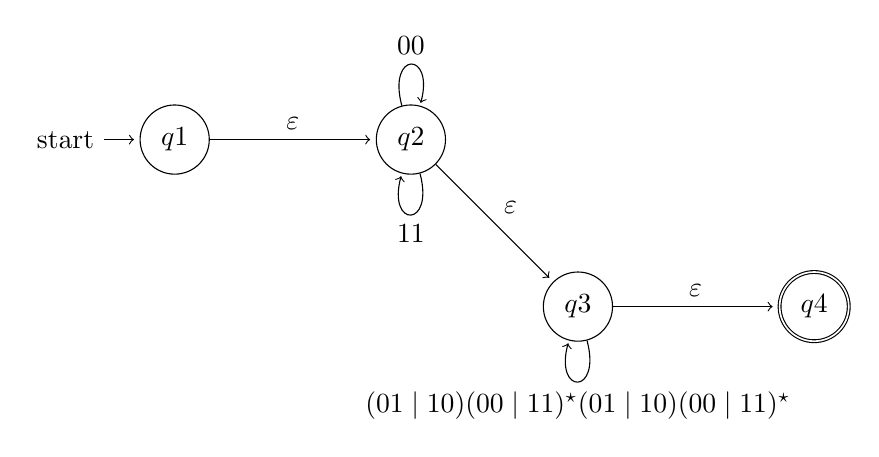
\begin{tikzpicture}[shorten >=2pt,node distance=3cm,on grid,auto] 
        \node[state,initial] (q_1)   {$q1$};  
        \node[state](q_2) [right=of q_1] {$q2$};
        \node[state](q_3) [below right=of q_2] {$q3$};
        \node[state,accepting](q_4) [right=of q_3] {$q4$};
        \path[->]
        (q_1) edge node {$\varepsilon$} (q_2)
        (q_2) edge node {$\varepsilon$} (q_3)
              edge [loop above] node {$00$} ()
              edge [loop below] node {$11$} ()
        (q_3) edge node {$\varepsilon$} (q_4)
              edge [loop below] node {$(01 \mid 10)(00 \mid 11)^{\star}(01 \mid 10)(00 \mid 11)^{\star}$} ();
      \end{tikzpicture}

\section{P63 第 9 题}
    {\large 对下面情况给出 DFA 及正规表达式。}

    \subsection{${0, 1}$ 上的含有子串 010 的所有串}

    \begin{tikzpicture}[shorten >=2pt,node distance=3cm,on grid,auto] 
      \node[state,initial] (q_1) {$q1$};  
      \node[state](q_2) [below right=of q_1] {$q2$};
      \node[state](q_3) [above right=of q_2] {$q3$};
      \node[state](q_4) [below right=of q_3] {$q4$};
      \node[state](q_5) [above right=of q_4] {$q5$};
      \node[state,accepting](q_6) [below right=of q_5] {$q6$};
      \path[->]
      (q_1) edge node {$\varepsilon$} (q_2)
      (q_2) edge node {$\varepsilon$} (q_3)
            edge [loop above] node {$0$} ()
            edge [loop below] node {$1$} ()
      (q_3) edge node {$010$} (q_4)
      (q_4) edge node {$\varepsilon$} (q_5)
      (q_5) edge node {$\varepsilon$} (q_6)
            edge [loop above] node {$0$} ()
            edge [loop below] node {$1$} ();
    \end{tikzpicture}

    \subsection{${0, 1}$ 上不含子串 010 的所有串}

    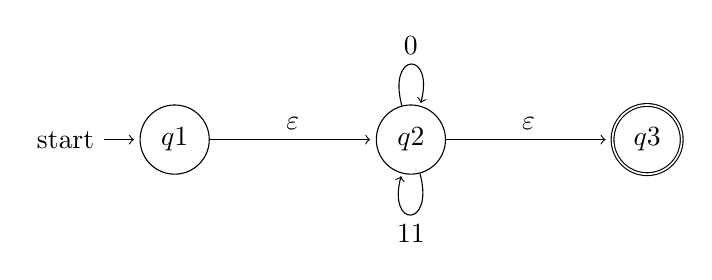
\begin{tikzpicture}[shorten >=2pt,node distance=3cm,on grid,auto] 
      \node[state,initial] (q_1) {$q1$};  
      \node[state](q_2) [right=of q_1] {$q2$};
      \node[state,accepting](q_3) [right=of q_2] {$q3$};
      \path[->]
      (q_1) edge node {$\varepsilon$} (q_2)
      (q_2) edge node {$\varepsilon$} (q_3)
            edge [loop above] node {$0$} ()
            edge [loop below] node {$11$} ();
    \end{tikzpicture}

\section{P63 第 12 题}
    \subsection{a 确定化与最小化}

    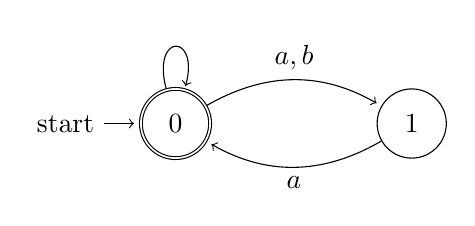
\begin{tikzpicture}[shorten >=2pt,node distance=3cm,on grid,auto] 
      \node[state,initial,accepting] (q_1)   {$0$};  
      \node[state](q_2) [right=of q_1] {$1$};
      \path[->] 
      (q_1) edge [bend left, above] node {$a, b$} (q_2)
            edge [loop above] node {} ()
      (q_2) edge [bend left, below] node {$a$} (q_1);
    \end{tikzpicture}

    {解:}\\

    \textbf{确定化}\\

    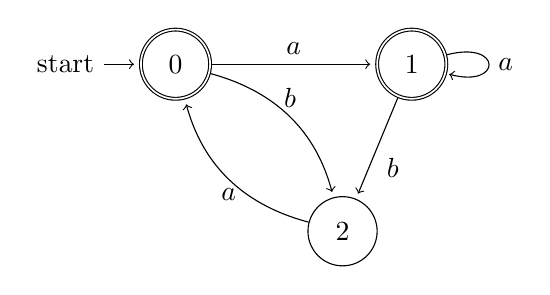
\begin{tikzpicture}[shorten >=2pt,node distance=3cm,on grid,auto] 
      \node[state,initial,accepting] (q_1)   {$0$};  
      \node[state,accepting](q_2) [right=of q_1] {$1$};
      \node[state](q_3) [below right=of q_1] {$2$};
      \path[->] 
      (q_1) edge node {$a$} (q_2)
            edge [bend left, above] node {$b$} (q_3)
      (q_2) edge node {$b$} (q_3)
            edge [loop right] node {$a$} ()
      (q_3) edge [bend left, below] node {$a$} (q_1);
    \end{tikzpicture}

    \textbf{最小化}\\

    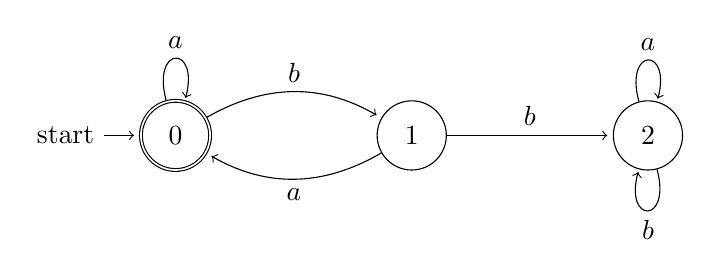
\begin{tikzpicture}[shorten >=2pt,node distance=3cm,on grid,auto] 
      \node[state,initial,accepting] (q_1) {$0$};
      \node[state] (q_2) [right=of q_1] {$1$};  
      \node[state] (q_3) [right=of q_2] {$2$};
      \path[->] 
      (q_1) edge [bend left, above] node {$b$} (q_2)
            edge [loop above] node {$a$} ()
      (q_2) edge [bend left, below] node {$a$} (q_1)
            edge node {$b$} (q_3)
      (q_3) edge [loop above] node {$a$} ()
            edge [loop below] node {$b$} ();
    \end{tikzpicture}

    \subsection{b 确定化与最小化}

    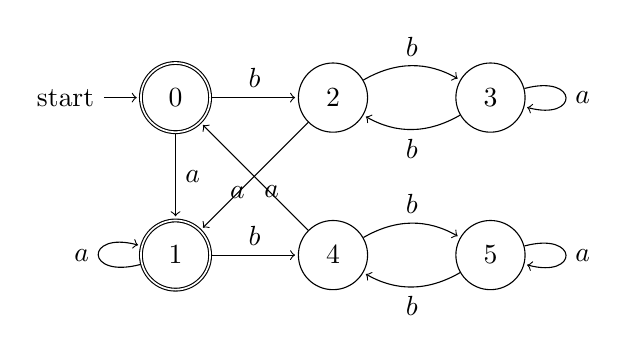
\begin{tikzpicture}[shorten >=1pt,node distance=2cm,on grid,auto] 
      \node[state,initial,accepting] (q_0) {$0$}; 
      \node[state,accepting] (q_1) [below=of q_0] {$1$}; 
      \node[state] (q_2) [right=of q_0] {$2$}; 
      \node[state] (q_3) [right=of q_2] {$3$}; 
      \node[state] (q_4) [right=of q_1] {$4$};
      \node[state] (q_5) [right=of q_4] {$5$};
      \path[->] 
      (q_0) edge node {$b$} (q_2)
            edge node {$a$} (q_1)
      (q_1) edge node {$b$} (q_4)
            edge [loop left] node {$a$} ()
      (q_2) edge [bend left, above] node {$b$} (q_3)
            edge node {$a$} (q_1)
      (q_3) edge [bend left, below] node {$b$} (q_2) 
            edge [loop right] node {$a$} ()
      (q_4) edge node {$a$} (q_0) 
            edge [bend left, above] node {$b$} (q_5)
      (q_5) edge [bend left, below] node {$b$} (q_4) 
            edge [loop right] node {$a$} ();
    \end{tikzpicture}

    \textbf{确定化}\\

    {显然此 NFA 已确定化。}\\

    \textbf{最小化}\\

    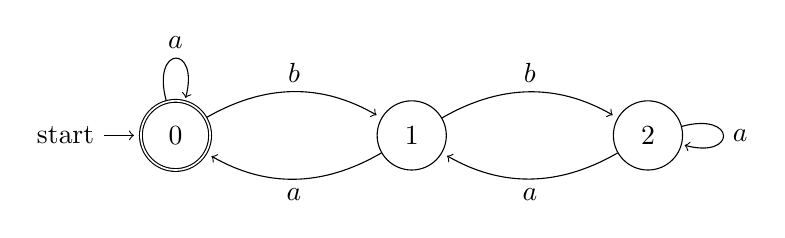
\begin{tikzpicture}[shorten >=2pt,node distance=3cm,on grid,auto] 
      \node[state,initial,accepting] (q_1) {$0$};
      \node[state] (q_2) [right=of q_1] {$1$};  
      \node[state] (q_3) [right=of q_2] {$2$};
      \path[->] 
      (q_1) edge [bend left, above] node {$b$} (q_2)
            edge [loop above] node {$a$} ()
      (q_2) edge [bend left, below] node {$a$} (q_1)
            edge [bend left, above] node {$b$} (q_3)
      (q_3) edge [loop right] node {$a$} ()
            edge [bend left, below] node {$a$} (q_2);
    \end{tikzpicture}

\end{document}